\documentclass[sigconfl]{acmart}

\usepackage{pdfpages}
\begin{document}

\title[Towards user-friendliness in proof assistants]{Towards user-friendliness
  in proof assistants: automated strategies \textbf{via} algebraic effects and handlers}

% \author{April Gonçalves}
% \email{april@metastate.dev}
% \affiliation{
%   \institution{Metastate}
%   \city{Edinburgh}
%   \state{UK}
% }

% \renewcommand{\shortauthors}{April Gonçalves}

\begin{abstract}
Proof assistants provide a framework for the modelling and verification of
theories, as well as trustworthy software. However, such power is usually only
available to experts. We propose a new approach, based on algebraic effects and
handlers, to integrate different automated proof strategies that enable
newcomers to take advantage of proof assistants without an in-depth
understanding of underlying theory. Our approach gives newcomers an effect
system, a handful of effectful strategies (tactics, proof search, and SMT
solvers) and their handlers under a shared interface, while advanced users can
extend our system with new effects and new handlers. Lastly, we prototype the
system as a library in Agda. While our prototype is minimal, it shows how easily
proofs can be carried out so long as the user has the correct intuition. We
believe our system empowers non-experts and has the potential to bring verified
software to many relevant industries, such as finance.
\end{abstract}

\keywords{effect handlers, proof assistants, user experience}

\maketitle

\section{Verification for the Masses}

The usability of proof assistants such as Coq, Agda, Isabelle/HOL and Twelf is
hard to measure: all of them require significant domain knowledge in type
theory, the theory that enables such assistants to exist. Coq and Isabelle/HOL
are more commonly applied outside their niche, and their programming style is
sharply different from
mainstream programming and even functional programming. Granted, they come with
their own integrated development environment (IDE), which may make it easier for
students and newcomers. To our knowledge, no usability study has been
held for a proof assistant, however there exists studies that account for
informal ``usability'' criteria -- they appear to measure how fast users can
familiarise themselves with the system or IDE.

Folklore within the proof assistants community says that newcomers
find Coq hard to use due to a large library of tactics and difficulty reading
the code after its completion. Many Coq learning materials suggest that users
add code comments for structural induction cases and inductive hypothesis. As
mentioned, no user studies were conducted to attest that such strategy improves
the perceived quality of Coq proofs.

Granted, proof assistants are a relatively new technology
and there are no guidelines or even an intuition on how such systems should
work or what features should be available to the users. The closest model we
have are proofs by hand. However, following that model for proof assistants has
two main pitfalls: (a) proofs by hand are not widely taught outside of
university mathematics courses; and (b) proof by hand and automated proof
employ fundamentally different paradigms, where the latter requires
axioms and formulations to be encoded explicitly, commonly known as a ``pedantic
proof style''.

\subsection{Empowering users of different levels of expertise}

To popularise software verification, we must make proof writing less of a
burden to the user. Currently, only specialists can write proofs for their
programs, even though the working programmer surely understands the domain and
invariants of their projects -- otherwise they would not be able to write any
software. \textit{Our hypothesis is that programmers are well-equipped to derive and
prove properties of the software they write, but they lack the mathematical maturity and
vocabulary to carry out a formal proof.} We have evidence that students fail to
produce well-made proofs due to the lack of mathematical maturity, even though
they do understand the subject matter at hand.

In our approach, we propose an effects and handlers view of such
proofs, based on prior work developed on the Andromeda proof assistant. Here,
our users will program as they would normally and invoke
the proof environment as an effect to prove certain properties as they go. Given
that the proof environment is \textit{just} an effect, we envision that different proof
styles (e.g., Agda-style dependent types, SMT solver, proof search) can be ``composed''
under a shared interface, a proof object that can manipulate itself while
querying different automated provers.

The reasons we employ algebraic effects and handlers are numerous:
\begin{enumerate}
\item as proofs cannot be fully automated, all approaches that try to automate
  the process (e.g, proof search, SMT solver) may be non-deterministic or
  never find a solution. Therefore, the system should be able to handle
  ``impure'' computations and errors. Algebraic effects and handlers have
  well-defined semantics and provide a simple interface for performing effects.
  With them, we avoid indiscriminate effects that are often error-prone and
  intricate effects machinery such as monad transformers;
\item the semantics of effects and handlers accommodate composition of arbitrary effects and the
  composition of multiple handlers, which means users have the ability to weaken
  more general strategies into specific ones while maintaining top-level
  handlers unmodified;
\item effects and handlers have well-defined semantics, and it is the main feature of many new
  research languages, such as Koka, Eff, Frank and Effekt, which suggests a greater
  potential due to their popularity.
\end{enumerate}

\subsection{Goals and Contributions}

The present project intends to be a compiler-level implementation as part of the
Juvix\footnote{Juvix is a dependently-typed programming language for smart
  contracts. More information at juvix.org} programming language. Juvix is designed
with focus on working programmers familiar with strongly-typed functional
programming.

\paragraph{Goals} The project exists to enable users to write safe, verified
code without investing time into learning dependent types and theorem proving.
The project's goals are to:
\begin{enumerate}
\item make software verification more accessible to programmers familiar with
  functional programming;
\item foster knowledge sharing between domain experts and regular programmers;
\item lower the barrier to entrance into software verification to non-experts.
\end{enumerate}

\paragraph{Contributions} The project is a work-in-progress, but this paper
makes three important contributions that pave the way for the full implementation:
\begin{enumerate}
\item a specification of a user interface for automated proofs based on
  algebraic effects and handlers that permits user-defined effects for proof
  strategies, and also user-defined handlers for existing effects (Section \ref{intro-witch});
\item a minimal prototype in Agda that validates the feasibility of such system
  (Section \ref{witch-agda});
\item a short technical account of the effort required to implement such a
  user interface for proof assistants (Section \ref{tech-details}).
\end{enumerate}

\section{Introducing Witch} \label{intro-witch}

\begin{figure}[!ht]
   \centering
    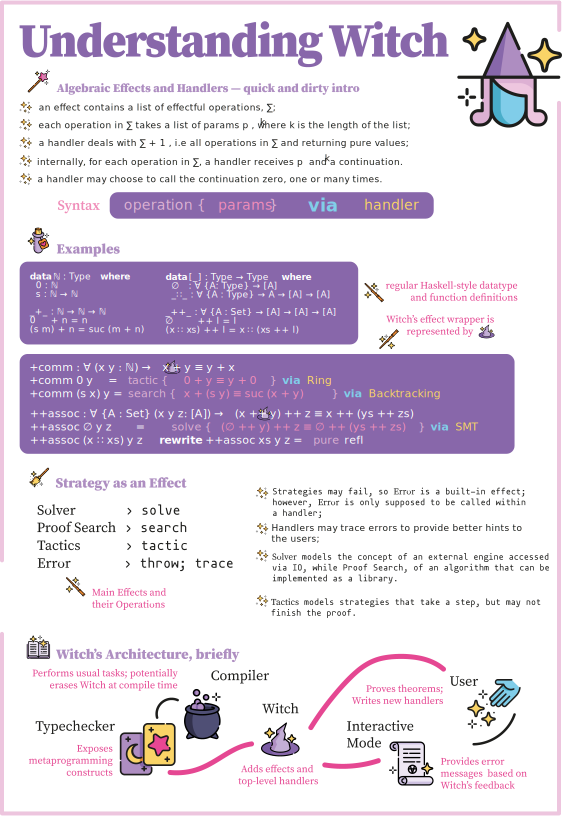
\includegraphics[height=\textheight]{image/witch.eps}
    \caption{Summary of Witch pertaining to strategies, examples
      and the architecture.}
    \label{fig:prototype}
\end{figure}

In this section, we introduce our approach, named Witch\footnote{Our tool's name is
  a play on the assistant tools colloquially called ``wizards''. There is no
  consensus of what a wizard is or what exactly the tasks are it is supposed
  assist with. Wizards seem to be used mostly for multiple-step and/or
  configuration features, however. We went for the name ``witch'' to align it to
  the idea of assistant tools, while dodging the overloaded, yet nebulous
  terminology.}. We define a \textit{witch} as an assistive tool for theorem
provers which congregates many different strategies for proof automation. Our
specification for a \textit{witch} for Juvix uses algebraic effects and handlers
as the means of congregation.

\paragraph{Algebraic Effects and Handlers} Algebraic effects were introduced by
**citation, and their handlers were introduced later on by **citation. An
algebraic effect is defined by a set of
operations, and handlers that denote said operations. A handler may interpret
operations at the compiler-level, which was formally named co-model, but
colloquially called ``top-level handler''. Handlers are the most general form to
denote a set of operations, and less general classes of handlers also exist.

\paragraph{The Essence of Witch}
In Figure \ref{fig:prototype}, we sum up our \textit{witch} approach.
As for the syntax, we use \texttt{operation \{ params \} via handler}, which is an
improvement over \texttt{handler(operation, params)}, since effect handling is similar
to function application, but also carries effect information.
The user defines data types and functions as usual, and then uses a
\textit{witch} to prove properties about said definitions. The Examples
section in Figure \ref{fig:prototype} shows this in action. The examples are
simplified for the sake of clarity -- we avoid
more complex properties and complicated proofs. The proof of
commutativity of addition under natural numbers and of associativity of list
concatenation are shown, and use the three main effects: Solver, Proof Search
and Tactics. In the proof assistant literature, there exists no precise
definition of commonly used terms ``solver'', ``proof search'' and ``tactics''.
All these terms are used in different communities, and mean some variation of
``automatic strategy to construct a term under certain constraints''. Here,
however, we use the following definitions:
\begin{itemize}
  \item The Solver effect is used for integration with external solvers via IO;
    we believe should suffice for the user to write, e.g. \texttt{SMT}, and handlers should
    implement internal strategies to choose between the different theories
    supported by solvers. If the black-box approach to solvers presents itself a
    challenge, a specialisation of the handler is possible, e.g.
    \texttt{operation \{ params \} via Z3.QF-UFLIA}.
  \item The Proof Search effect is used for library-level algorithms; users may
    choose to implement their own algorithms using a limited set of
    meta-programming\footnote{By meta-programming, we mean ``code that manipulates
    itself'', and not ``programming that happens in a higher level of abstraction''.
    For dependently typed programming languages, the usual term is reflection.
    However, we prefer not use reflection since it has another meaning in
    terms of effectful computations.} constructs that are handled at top-level\footnote{The
      meta-programming constructs are operations of the Typechecker effect
      whose handlers are not available for the user.}.
  \item The Tactics effect is used for strategies that simplify the goal at
    least one step, and may not complete all proof goals. This style is mainly
    used in the proof assistant Coq. While we do not foresee using as many as many
    tactics implemented as in Coq, we believe tactics such as
    \texttt{eauto}, \texttt{??}, \texttt{??} are useful to users of
    all levels of expertise.
    \item Lastly, the Error effect is used for feedback to the user,
    since any of the strategies may fail. Error has two operations,
    \texttt{throw} and \texttt{trace}: the former notifies the user that a strategy
    has failed, while the latter registers\footnote{Internally, the
      Typechecker effect should have a tree that stores all currently
      saved traces.} completed sub-goals during the
    strategy's attempt to complete the proof.
\end{itemize}

\paragraph{Witch's Architecture}
A \textit{witch} sits between the typechecker and the interactive mode of a
proof assistant. It uses meta-programming constructs provided by the typechecker and notifies
the interactive mode about whether the current attempted strategy was successful.
The user may manipulate proof handlers by composing or writing their own.


\paragraph{Downsides of our Approach}
There are two main styles for writing proofs within a proof assistant: external
verification and internal verification. The latter encourages code
that is \textit{correct-by-construction}, meaning only valid states can be
encoded and values carry all information necessary to make proofs trivial; while
the former encourages writing code as usual, and reconstructing information
needed for proofs only when necessary.
Witch's primarily focus is on external verification. We believe that newcomers
will struggle to write proof-aware code, since it departs strongly from
mainstream programming, even within the functional style. We expect users to
write their code as they normally would do and then prove necessary properties.
Witch does not support writing correct-by-construction code. As proofs
are erased during compilation-time in Juvix, Witch could be extended
to be indexed by proof objects and parameterised over any type, such as
\texttt{\{A: Type\} $\rightarrow$ x y: A $\rightarrow$ }
\includegraphics[height=0.02\textheight]{image/hat.eps} \texttt{ (x * y $\equiv$
  y * x) }.


\section{Agda's Witch} \label{witch-agda}

\paragraph{Why Agda?} Agda provides higher-level meta-programming constructs, and
its coding style is a reminiscent of the ML family of functional programming languages.

\subsection{Technical Effort Required} \label{tech-details}

Although Witch can be implemented as a library, it requires certain features
from the proof assistant. The most important feature is type-level
meta-programming: Witch requires that the proof assistant can manipulate its own
proof terms, generate new variables, holes, goals, among others, and manipulate
terms and types in a type-safe fashion.
Secondly, the proof assistant should provide an interface to the outside world
while type checking
It is not essential, its absence means that no external solver can be
integrated, diminishing the value of the tool.
Lastly, the proof assistant must support algebraic effects and handlers. If there
is no built-in solution, a library-level solution is possible -- as we did in
Agda. However, a solid implementation may not be trivial to achieve. In Agda,
we translate effect handling into optimised continuation-passing style that inlines
all applications. This strategy can also be implemented at the compiler-level,
if necessary. There are many strategies to efficiently implement algebraic
effects and handlers, but we opted for the one that seemed the most
straight-forward method to implement it in Agda.

\section{Related and Future Work}

\subsection{Comparison with Similar Approaches}

\paragraph{Andromeda proof assistant} As mentioned, this project was inspired by the
Andromeda proof assistant. It follows the LCF tradition of theorem provers,
where there exist two distinct languages. One habits a safe nucleus that
verifies hypotheses, on the other hand, the second hand comprises a polymorphic
$\lambda$ calculus where users implement their theories and relay the
verification to the nucleus.

\paragraph{Meta-F*} F* is a dependently typed language with (monadic) effects and liquid
types. For tactics, F* uses a library called Meta-F*, where tactics are
considered an effect that uses meta-programming provided by the typechecker to
manipulate proof objects. Agda's Witch implementation is heavily inspired by Meta-F*.

\paragraph{Mtac and Cybele} The idea of proof strategies happening within an
effectful structure was first introduced in Cybele and later extended into Mtac.
Mtac extends Coq's powerful main language, providing the user with a
dependently-typed tactic language.

\subsection{Improving Witch Further}
While it is hard to say whether we have achieved our goals before user
evaluations, Witch is a first step towards a future where proof assistants are
friendlier to users, particularly newcomers. The present work is in its
infancy, and there are many open problems regarding Witch's ability to guide newcomers
towards correct-by-construction software, which constitutes the main improvement
we intend for Witch. We hypothesise possibility of inserting into the source
code a  \textit{proof sketch} that contains sub-goals of interest for the user and guides the
typechecker to rebuild the derivation tree faster. This change would, therefore,
relocate Witch to an assistant that lives solely
within the interactive mode -- as opposed to a framework for proof
automation in user code. The implementation of such feature may present itself
as a challenge, however.

In parallel with the usability work, we plan to develop a formalisation of Witch
as a dependent typed language with effectful, dependently typed operations and
effect handler, based on previous work on fibred algebraic effects.

\end{document}
\endinput
